% ============================================================
% PHẦN 3.4 — CHÂN DUNG KHÁCH HÀNG ĐIỂN HÌNH
% ------------------------------------------------------------
% Thuộc: PA3-01
% Người phụ trách chính: Trần Minh Quang – Marketing Lead
% Phối hợp: Nguyễn Anh Thư
%
% CÂU HỎI CẦN TRẢ LỜI:
%   - Ai là người duyệt ngân sách?
%   - Ai là người sử dụng trực tiếp sản phẩm?
%   - Ai cung cấp dữ liệu khóa học cho hệ thống?
%   - Khách hàng cần có bao nhiêu nhân sự marketing, livestream và tư vấn?
%   - Nội dung nào thường xuyên bị lặp lại: học phí, lịch học, đầu vào, ưu đãi, học thử hay chính sách?
%
% OUTPUT BẮT BUỘC:
%   1. Chân dung người MUA HÀNG (Buying Persona):
%      - Ví dụ: Chủ trung tâm hoặc quản lý chi nhánh
%      - Mục tiêu kinh doanh
%      - Vấn đề
%      - Rào cản
%      - Tiêu chí mua
%      - Kênh thường tiếp nhận thông tin
%
%   2. Chân dung người DÙNG TRỰC TIẾP (User Persona):
%      - Ví dụ: Trưởng marketing / Nhân viên nội dung /
%               Tư vấn tuyển sinh / Nhân viên trực livestream
%
%   3. Bảng đơn vị ra quyết định mua (Buying Center):
%      - Vai trò | Chức danh | Mối quan tâm |
%        Thông điệp cần truyền đạt | Kênh tiếp cận phù hợp
%
% LƯU Ý:
%   Business Plan đã phân biệt:
%     - Người duyệt ngân sách
%     - Người bảo trợ nội bộ
%     - Người sử dụng trực tiếp
%     - Người cung cấp dữ liệu
%     - Người có thể phản đối
%   PA3 cần sử dụng lại cấu trúc này khi xây dựng thông điệp và kênh tiếp cận.
%
% TIÊU CHÍ HOÀN THÀNH:
%   - Persona phải có hành vi, vấn đề và tiêu chí quyết định mua
%   - Thông tin chưa kiểm chứng phải ghi rõ là GIẢ ĐỊNH
% ============================================================

\subsection{Chân dung khách hàng điển hình}

\textbf{Báo cáo Nghiên cứu Chiến lược Tiếp cận Thị trường (Go-To-Market) cho Giải pháp AI Livestream Lĩnh vực Giáo dục}

Bối cảnh chuyển đổi số trong nền kinh tế số và đặc biệt là lĩnh vực giáo dục tại Việt Nam đang diễn ra với tốc độ chưa từng có, định hình lại toàn bộ phương thức tiếp cận và tương tác với học viên. Theo các phân tích thị trường giáo dục công nghệ (EdTech) mới nhất, Việt Nam hiện nằm trong top 10 thị trường EdTech phát triển nhanh nhất thế giới và top 3 tại khu vực Đông Nam Á.\footnote{Việt Nam nằm trong top 10 thị trường EdTech thế giới, top 3 thị trường Đông Nam Á, accessed July 17, 2026, \url{https://vneconomy.vn/techconnect/viet-nam-nam-trong-top-10-thi-truong-edtech-the-gioi-top-3-thi-truong-dong-nam-a.htm}} Đáng chú ý, quy mô thị trường giáo dục trực tuyến K-12 toàn cầu dự kiến sẽ tăng vọt từ 107,5 tỷ USD năm 2023 lên 755,1 tỷ USD vào năm 2030.\footnote{Quy mô thị trường giáo dục trực tuyến K-12, Báo cáo xu hướng ngành, accessed July 17, 2026, \url{https://www.forinsightsconsultancy.com/vi/b\%C3\%A1o-c\%C3\%A1o/th\%E1\%BB\%8B-tr\%C6\%B0\%E1\%BB\%9Dng-gi\%C3\%A1o-d\%E1\%BB\%A5c-tr\%E1\%BB\%B1c-tuy\%E1\%BA\%BFn-k-12}} Sự bùng nổ của thương mại điện tử qua video (Video Commerce) tại khu vực Đông Nam Á, với mức tăng trưởng Tổng giá trị giao dịch (GMV) gấp 2,5 lần trong hai năm qua và chiếm tới 25\% tổng GMV thương mại điện tử\footnote{Nguồn: [CSH2026][1Stream][FINAL PITCH DECK].pdf}, đã mở ra một kỷ nguyên mới. Hơn 67\% chi tiêu trực tuyến tại Việt Nam hiện được thúc đẩy trực tiếp thông qua các phiên livestream.\footnote{Nguồn: [CSH2026][1Stream][FINAL PITCH DECK].pdf}

Tuy nhiên, việc vận hành kênh livestream bán khóa học và tư vấn tuyển sinh đang vấp phải rào cản khổng lồ về mặt chi phí và hiệu suất. Cấu trúc chi phí vận hành của các trung tâm giáo dục đang mất cân đối nghiêm trọng, trong đó chi phí nhân sự chiếm từ 50\% đến 60\% tổng chi phí hoạt động.\footnote{Nguồn: [CSH2026][1Stream][FINAL PITCH DECK].pdf} Trong bối cảnh nguồn vốn đầu tư mạo hiểm (VC) vào EdTech toàn cầu đang cho thấy sự chắt lọc khắt khe hơn (đạt 2,4 tỷ USD vào năm 2024 với 342 giao dịch)\footnote{Sách trắng EdTech Việt Nam 2025 | PDF -- Scribd, accessed July 17, 2026, \url{https://www.scribd.com/document/996258987/Sa-ch-tra-ng-EdTech-Vi\%E1\%BB\%87t-Nam-2025}}, các doanh nghiệp giáo dục buộc phải tìm kiếm các giải pháp công nghệ tự động hóa, cụ thể là trí tuệ nhân tạo (AI), để tối ưu hóa biên lợi nhuận.

Báo cáo nghiên cứu chiến lược này được biên soạn nhằm phân tích toàn diện và giải quyết triệt để 5 câu hỏi trọng tâm về định vị nhân sự, cấu trúc vận hành, và hệ sinh thái nội dung tại các trung tâm giáo dục/ngoại ngữ. Trên cơ sở phân tích thực chứng, báo cáo phác họa chi tiết Chân dung Người mua hàng (Buying Persona), Chân dung Người dùng trực tiếp (User Persona) và Bảng Đơn vị ra quyết định mua (Buying Center) dưới lăng kính chiến lược Tiếp cận thị trường (Go-To-Market -- GTM). Kết quả của báo cáo sẽ đóng vai trò như một bản thiết kế (blueprint) để định hướng các chiến dịch marketing B2B cho giải pháp phần mềm dạng dịch vụ (SaaS) ứng dụng AI trong quản lý livestream giáo dục.

%% ================================================================
%% PHẦN 1: PHÂN TÍCH CHUYÊN SÂU
%% ================================================================
\subsubsection{Phần 1: Phân tích Chuyên sâu và Giải đáp 5 Câu hỏi Trọng tâm của Thị trường}

Để thiết kế một chiến lược GTM sắc bén, việc thấu hiểu cơ chế vận hành nội bộ của khách hàng mục tiêu (các trung tâm ngoại ngữ, hệ thống giáo dục tư thục) là điều kiện tiên quyết. Các phân tích dưới đây sẽ bóc tách từng lớp cấu trúc quyền lực, luồng công việc và hành vi của hệ sinh thái này.

\paragraph{1. Ai là người duyệt ngân sách?}

Trong cấu trúc tổ chức và quản trị trị học thuật của các cơ sở đào tạo giáo dục tại Việt Nam, quy trình ra quyết định mua sắm (procurement decision) mang tính tập trung cao độ. Người nắm giữ quyền quyết định cuối cùng về việc phân bổ nguồn vốn đầu tư công nghệ mới, mua sắm phần mềm SaaS là \textbf{Giám đốc trung tâm}, \textbf{Chủ đầu tư (Founder/Co-founder)}, hoặc \textbf{Giám đốc/Quản lý chi nhánh} (đối với các hệ thống chuỗi có mức độ phân quyền tài chính nhất định).\footnote{Cấu trúc nhân sự trung tâm ngoại ngữ: Giám đốc, giáo viên và các bộ phận chuyên môn, accessed July 17, 2026, \url{https://luatminhthinh.vn/cau-truc-nhan-su-trung-tam-ngoai-ngu-giam-doc-giao-vien-va-cac-bo-phan-chuyen-mon/}}

Quyết định giải ngân của nhóm đối tượng cấp cao này hiếm khi dựa trên các yếu tố công nghệ đơn thuần (như thuật toán AI hay tính năng phần mềm), mà được thúc đẩy mạnh mẽ bởi bài toán tài chính vi mô: tối ưu hóa lợi nhuận (Profit Margin) và cắt giảm chi phí hoạt động (OPEX). Theo các dữ liệu thống kê hiện hành, chi phí nguồn nhân lực để duy trì hoạt động kinh doanh trực tuyến, đặc biệt là đội ngũ trực page, trực livestream ngoài giờ hành chính đang nuốt trọn 50\% đến 60\% ngân sách vận hành của các nhà bán hàng và trung tâm giáo dục.\footnote{Nguồn: [CSH2026][1Stream][FINAL PITCH DECK].pdf} Người duyệt ngân sách chịu áp lực trực tiếp từ các mục tiêu kinh doanh vĩ mô. Khi đánh giá một giải pháp AI, họ không mua một ``phần mềm'', mà họ đang mua một ``giải pháp cắt giảm chi phí nhân sự ngoài giờ'' và ``công cụ gia tăng tỷ lệ chuyển đổi học viên (Conversion Rate) trên mỗi phiên live''.

Ngoài ra, quá trình phê duyệt không phải lúc nào cũng mang tính độc đoán. Tại các trung tâm quy mô trung bình đến lớn, Giám đốc trung tâm có thẩm quyền thành lập các hội đồng tư vấn (bao gồm các Trưởng phòng chuyên môn như Marketing, Đào tạo, Hành chính -- Nhân sự) để đánh giá tính khả thi của giải pháp công nghệ trước khi chính thức đưa ra quyết định.\footnote{Điều kiện của bộ máy nhân sự trung tâm ngoại ngữ -- Luật Thành Đô, accessed July 17, 2026, \url{https://luatthanhdo.com.vn/dieu-kien-cua-bo-may-nhan-su-trung-tam-ngoai-ngu}} Do đó, người duyệt ngân sách phụ thuộc rất nhiều vào các báo cáo đánh giá hiệu quả đầu tư (ROI) do cấp dưới đệ trình. Họ cần nhìn thấy một lộ trình hoàn vốn (Payback period) rõ ràng, thường được kỳ vọng trong vòng dưới 6 tháng đối với các mô hình SaaS B2B.

\begin{figure}[H]
    \centering
    
\includegraphics[width=0.85\linewidth]{imgs/PA3_pics/image1_v3.png}
    \caption{Quy trình phê duyệt ngân sách và cấu trúc tổ chức tại trung tâm giáo dục}
    \label{fig:pa3_budget_approval}
\end{figure}

\paragraph{2. Ai là người sử dụng trực tiếp sản phẩm?}

Một hệ thống nền tảng quản lý livestream đa kênh tích hợp AI tư vấn chốt đơn\footnote{Nguồn: [CSH2026][1Stream][FINAL PITCH DECK].pdf} không phải là một công cụ đơn lẻ mà là một trung tâm điều phối (hub) yêu cầu sự tương tác trực tiếp và liên tục của nhiều phòng ban khác nhau trong một vòng đời bán hàng (sales cycle) hoàn chỉnh. Những người dùng trực tiếp (Direct Users) cấu thành nên hệ sinh thái người dùng bao gồm:

\begin{itemize}
    \item \textbf{Nhân viên Vận hành Livestream / Content Creator / Host:} Họ là những người thao tác trực tiếp trên giao diện (dashboard) của phần mềm trong thời gian thực. Công việc của họ bao gồm việc thiết lập phiên live, tinh chỉnh hình ảnh, phối hợp kịch bản (cùng với bộ phận học thuật) và đảm bảo luồng phát sóng ổn định trên các nền tảng như TikTok, Facebook, YouTube.\footnote{Giáo viên Tiếng Anh Host Livestream -- Joboko, accessed July 17, 2026, \url{https://vn.joboko.com/viec-lam-giao-vien-tieng-anh-host-livestream-xvi6575019?amp=1}} Áp lực của họ là duy trì năng lượng liên tục trong các phiên live kéo dài.
    \item \textbf{Trưởng phòng / Chuyên viên Marketing (Digital Marketing):} Nhóm này sử dụng hệ thống như một công cụ đo lường và tối ưu hóa. Họ phân tích báo cáo hiệu suất (Analytics \& Dashboard), theo dõi số lượng bình luận chưa xử lý, tốc độ phản hồi của AI và con người, từ đó phân tích dữ liệu về ý định mua (intent) của học viên để điều chỉnh các chiến dịch quảng cáo, ưu đãi trong tương lai.\footnote{Nguồn: [CSH2026][1Stream][FINAL PITCH DECK].pdf}
    \item \textbf{Nhân viên Tư vấn tuyển sinh (Telesales / Education Consultants):} Đây là lực lượng nòng cốt tạo ra doanh thu. Khi hệ thống AI Sales Agent thực hiện bước lọc phễu ban đầu (phân loại bình luận, trả lời các câu hỏi cơ bản), hoặc phát hiện các ``intent'' chốt đơn cao, các câu hỏi phức tạp vượt ngoài khả năng của bộ quy tắc AI (rule-based logic), hệ thống sẽ chuyển giao cuộc hội thoại cho nhân viên tư vấn.\footnote{Nguồn: [CSH2026][1Stream][FINAL PITCH DECK].pdf} Nhóm này tương tác trực tiếp với giao diện quản lý hội thoại đa kênh để thực hiện nghiệp vụ chốt sales, chăm sóc khách hàng và thuyết phục học viên.\footnote{Tuyển dụng NHÂN VIÊN TƯ VẤN TUYỂN SINH TRUNG TÂM TIẾNG ANH tại Hà Nội, accessed July 17, 2026, \url{https://viecoi.vn/viec-lam/nhan-vien-tu-van-tuyen-sinh-trung-tam-tieng-anh-45976.html}}
\end{itemize}

Sự chồng chéo và đa dạng trong hành vi của những người sử dụng trực tiếp này đặt ra một yêu cầu khắt khe về mặt phát triển sản phẩm: giải pháp công nghệ phải sở hữu giao diện trực quan (UI), trải nghiệm người dùng (UX) tối giản, học hỏi nhanh (low learning curve) và không đòi hỏi trình độ IT chuyên sâu để vận hành. Nếu hệ thống quá phức tạp, nó sẽ đối mặt với sự phản kháng ngầm (internal resistance) từ chính đội ngũ nhân viên, dẫn đến tỷ lệ rời bỏ (churn rate) cao.

\paragraph{3. Ai cung cấp dữ liệu khóa học cho hệ thống?}

Bất kỳ một hệ thống AI bán hàng (Sales Agent), Chatbot hay nền tảng tạo video tự động (Video Generator) nào cũng hoạt động dựa trên nguyên lý ``Garbage In, Garbage Out'' (Dữ liệu đầu vào kém sẽ cho ra kết quả kém). Hiệu quả, tính chính xác và mức độ thông minh của hệ thống AI hoàn toàn phụ thuộc vào chất lượng, tính toàn vẹn và độ cập nhật của Cơ sở dữ liệu tri thức (Knowledge Database).\footnote{Nguồn: [CSH2026][1Stream][FINAL PITCH DECK].pdf} Những mắt xích chịu trách nhiệm cung cấp, chuẩn hóa và hiệu đính nguồn dữ liệu quan trọng này bao gồm:

\begin{itemize}
    \item \textbf{Bộ phận Học vụ / Trưởng phòng Đào tạo (Academic Department):} Họ là những người nắm giữ ``linh hồn'' của trung tâm. Nhóm này chịu trách nhiệm cung cấp thông tin học thuật chuẩn xác, cấu trúc khóa học, phương pháp giảng dạy (ví dụ: phương pháp NLP, PPP, TBLT)\footnote{[Mới Nhất] TOP 10 TRUNG TÂM TIẾNG ANH CHO NGƯỜI ĐI LÀM TẠI ĐÀ NẴNG, accessed July 17, 2026, \url{https://wiseenglish.edu.vn/trung-tam-tieng-anh-cho-nguoi-di-lam}}, lộ trình đầu vào/đầu ra, cam kết điểm số và lịch trình khai giảng chi tiết.\footnote{Học Viên Hỏi -- Chatbot Trả Lời: Gỡ Tắc Nghẽn Thông Tin Học Vụ -- NIXXIS, accessed July 17, 2026, \url{https://nixxis.vn/chatbot-tu-van-hoc-vu-cho-hoc-vien/}}
    \item \textbf{Quản lý Khóa học / Cán bộ Hành chính (Operations / Admin):} Nhóm này đóng vai trò cung cấp các biểu giá (học phí) được cập nhật mới nhất, các chính sách ưu đãi theo từng chiến dịch, chính sách bảo lưu, chuyển lớp, hoặc quy định hoàn trả học phí.
    \item \textbf{Giáo viên / Chuyên gia chuyên môn (Teachers / Subject Matter Experts):} Họ cung cấp chiều sâu cho dữ liệu. Giáo viên trực tiếp đóng góp các kiến thức chuyên ngành để đào tạo AI (train the model) cách trả lời các câu hỏi kỹ thuật hóc búa của học viên về ngữ pháp, phát âm (IPA), từ vựng chuyên ngành hoặc cấu trúc bài thi quốc tế (IELTS, TOEIC, SAT).\footnote{Giáo viên Tiếng Anh Host Livestream -- Joboko, accessed July 17, 2026, \url{https://vn.joboko.com/viec-lam-giao-vien-tieng-anh-host-livestream-xvi6575019?amp=1}}
\end{itemize}

Việc thu thập và chuẩn hóa hàng loạt dữ liệu từ các tệp Excel, Word, PDF rời rạc hay thậm chí từ những cuốn cẩm nang nội bộ thành một bộ Knowledge Base có cấu trúc (ví dụ: định dạng JSON) là một quy trình mang tính sống còn. Điều này cho phép hệ thống áp dụng các thuật toán truy xuất tiên tiến như Tìm kiếm Vector, TF-IDF hoặc RAG (Retrieval-Augmented Generation).\footnote{Nguồn: [CSH2026][1Stream][FINAL PITCH DECK].pdf} Cơ chế RAG đặc biệt quan trọng vì nó buộc AI ngôn ngữ lớn (LLM) chỉ được phép trích xuất câu trả lời từ chính nguồn tài liệu do trung tâm cung cấp, qua đó triệt tiêu hoàn toàn rủi ro AI tự huyễn hoặc (hallucination) -- sinh ra các thông tin sai lệch về giá cả hay cam kết đầu ra gây tổn hại nghiêm trọng đến uy tín thương hiệu.

\paragraph{4. Khách hàng cần có bao nhiêu nhân sự marketing, livestream và tư vấn?}

Quy mô và cơ cấu nhân sự phục vụ cho công tác marketing, vận hành kênh livestream và tư vấn tuyển sinh không có một mẫu số chung mà biến động vô cùng mạnh mẽ, phụ thuộc hoàn toàn vào quy mô hoạt động, dòng tiền và chiến lược thâm nhập thị trường của từng tổ chức giáo dục. Sự phân hóa này tạo ra các nhóm nhu cầu ứng dụng công nghệ (use-cases) rất khác biệt.

\begin{itemize}
    \item \textbf{Đối với các Hệ thống giáo dục và Trung tâm ngoại ngữ quy mô trung bình đến lớn:} Cơ cấu tổ chức tại đây được phân bổ rất chuyên biệt, sở hữu nguồn lực mạnh và bộ máy đồ sộ. Theo một báo cáo phân tích hoạt động nhân sự tại một công ty giáo dục, một phòng Marketing tiêu chuẩn có thể duy trì tới 11 nhân sự cơ hữu (bao gồm 1 Trưởng phòng, 2 nhân viên phụ trách Fanpage, 2 nhân viên quản trị Website/SEO, 2 nhân viên chuyên trách mảng TikTok, 2 chuyên viên nghiên cứu thị trường, và 2 nhân viên tổ chức sự kiện).\footnote{Báo Cáo Thực Tập Tổng Hợp K57C -- Nguyễn Thị Hảo, ĐH Thương Mại, accessed July 17, 2026, \url{https://www.studocu.vn/vn/document/truong-dai-hoc-thuong-mai/phan-tich-bctc/27lop57c2nguyen-thi-hao-bctttn/107980845}}
    \begin{itemize}
        \item Trong khi đó, bộ phận tư vấn tuyển sinh thường hoạt động độc lập dưới quyền của một Trưởng nhóm hoặc Trưởng phòng Tư vấn tuyển sinh, quản lý một đội ngũ từ 3 đến 10 chuyên viên (Telesales/Consultants) tùy thuộc vào số lượng cơ sở (branch) và chỉ tiêu doanh số hàng tháng.\footnote{CÔNG TY TRÁCH NHIỆM HỮU HẠN TRUNG TÂM NGOẠI NGỮ AMA VŨNG TÀU tuyển dụng Trưởng phòng Tư vấn tuyển sinh -- UEH Youth, accessed July 17, 2026, \url{https://youth.ueh.edu.vn/ho-tro-sinh-vien-2/cong-ty-trach-nhiem-huu-han-trung-tam-ngoai-ngu-ama-vung-tau-tuyen-dung-truong-phong-tu-van-tuyen-sinh/}}
        \item Để vận hành một phòng livestream chuyên nghiệp với các phiên live dài, họ cần tuyển dụng ít nhất 1--2 Host livestream (thường là các giáo viên tiếng Anh có ngoại hình sáng, khả năng hoạt ngôn, phát âm chuẩn IPA) và 1 đến 2 nhân viên kỹ thuật vận hành luồng live, setup ánh sáng, điều khiển các nền tảng phát sóng.\footnote{Giáo viên Tiếng Anh Host Livestream -- Joboko, accessed July 17, 2026, \url{https://vn.joboko.com/viec-lam-giao-vien-tieng-anh-host-livestream-xvi6575019?amp=1}} Mức thu nhập cho một nhân sự Host livestream tiếng Anh chuyên nghiệp dao động từ 10 -- 20 triệu/tháng, có thể lên tới 50 triệu nếu gắn với KPI doanh số khổng lồ.\footnote{Giáo viên Tiếng Anh Host Livestream -- Joboko, accessed July 17, 2026, \url{https://vn.joboko.com/viec-lam-giao-vien-tieng-anh-host-livestream-xvi6575019}}
    \end{itemize}
    \item \textbf{Đối với các Trung tâm nhỏ (SME), Micro-seller và Giáo viên dạy độc lập:} Nguồn lực của nhóm này vô cùng hạn chế, dẫn đến mô hình hoạt động ``đa nhiệm'' (multi-tasking). Dựa trên bối cảnh thị trường thực tế (GIẢ ĐỊNH từ xu hướng micro-business), nhóm này thường chỉ có 1 đến 2 nhân sự kiêm nhiệm gần như mọi vai trò. Một giáo viên sáng lập trung tâm có thể vừa đứng lớp giảng dạy ban ngày, vừa tự setup đèn đóm và đóng vai trò Host livestream vào buổi tối muộn (ví dụ: bắt đầu phiên live lúc 20:00).\footnote{Chi chục triệu học livestream bán hàng -- Báo Tuổi Trẻ, accessed July 17, 2026, \url{https://tuoitre.vn/nld/chi-chuc-trieu-hoc-livestream-ban-hang-196231203114313834.htm}} Trong khi đó, một nhân viên hành chính duy nhất (hoặc chính vợ/chồng của chủ trung tâm) sẽ đảm nhận cùng lúc việc gõ máy tính trực bình luận, lọc tin nhắn và chốt sale.\footnote{Giáo viên Tiếng Anh Host Livestream -- Joboko, accessed July 17, 2026, \url{https://vn.joboko.com/viec-lam-giao-vien-tieng-anh-host-livestream-xvi6575019}}
    \begin{itemize}
        \item Chi phí để bước chân vào sân chơi livestream cũng không hề nhỏ đối với nhóm SME. Một khóa học dạy kỹ năng livestream bán hàng chuyên nghiệp có thể tốn gần 10 triệu đồng, đi kèm với chi phí thiết lập phòng live, ánh sáng, máy quay tiêu tốn thêm khoảng 30 triệu đồng.\footnote{Chi chục triệu học livestream bán hàng -- Báo Tuổi Trẻ, accessed July 17, 2026, \url{https://tuoitre.vn/nld/chi-chuc-trieu-hoc-livestream-ban-hang-196231203114313834.htm}}
        \item Theo GIẢ ĐỊNH dựa trên chi phí vận hành, những trung tâm nhỏ lẻ này không thể chịu nổi nhiệt để trả mức lương trung bình 15--25 triệu/tháng cho một đội ngũ nhân sự tư vấn chuyên biệt hay Host livestream chuyên nghiệp.\footnote{Việc làm Nhân viên tư vấn trung tâm ngoại ngữ -- Indeed, accessed July 17, 2026, \url{https://vn.indeed.com/q-nh\%C3\%A2n-vi\%C3\%AAn-t\%C6\%B0-v\%E1\%BA\%A5n-trung-t\%C3\%A2m-ngo\%E1\%BA\%A1i-ng\%E1\%BB\%AF-vi\%E1\%BB\%87c-l\%C3\%A0m.html}} Hậu quả là, khi một phiên livestream bất ngờ lọt vào xu hướng (trending) và lượng bình luận tăng vọt, nhóm SME lập tức vỡ trận, đối mặt với rủi ro bỏ sót khách hàng (lead leakage) rất cao, lãng phí hoàn toàn chi phí quảng cáo và nỗ lực làm nội dung.
    \end{itemize}
\end{itemize}

\begin{figure}[H]
    \centering
    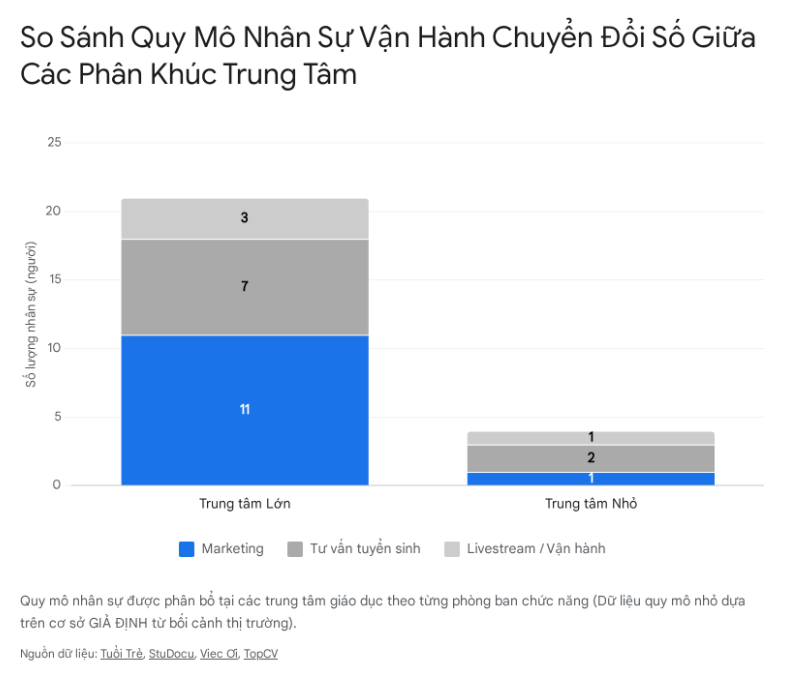
\includegraphics[width=0.85\linewidth]{imgs/PA3_pics/image2_v3.png}
    \caption{So sánh mô hình nhân sự giữa trung tâm quy mô lớn và trung tâm nhỏ}
    \label{fig:pa3_staffing_comparison}
\end{figure}

\paragraph{5. Nội dung nào thường xuyên bị lặp lại trong các phiên tiếp thị?}

Hành trình khách hàng (Customer Journey) trong mảng giáo dục đào tạo, đặc biệt là việc đăng ký các khóa học ngôn ngữ, là một chuỗi quyết định đòi hỏi sự cân nhắc kỹ lưỡng (high-involvement decision). Tuy nhiên, vòng đời ra quyết định của học viên thường bắt đầu bằng vô số các truy vấn mang tính thông tin cơ bản trước khi họ thực sự chuyển sang giai đoạn cân nhắc và mua hàng. Phân tích dữ liệu học thuật, hoạt động tư vấn và các luồng bình luận trên mạng xã hội cho thấy các nhóm nội dung bị lặp lại với tần suất dày đặc nhất bao gồm:

\begin{enumerate}
    \item \textbf{Học phí (Tuition Fees):} Đây là câu hỏi kinh điển, phổ biến nhất và có tính cấu trúc cao nhất. Bất chấp việc thông tin có thể đã được ghim trên màn hình, học viên vẫn liên tục hỏi trên livestream hoặc chat. Mức độ phức tạp của câu hỏi này nằm ở chỗ học phí có độ dao động rất lớn. Chẳng hạn, khảo sát cho thấy học phí các khóa IELTS thường dao động từ 5.920.000 VNĐ đến 17.000.000 VNĐ tùy theo lộ trình và đầu vào.\footnote{Khoá học IELTS cơ bản, học phí từ 5.920.000 -- Trung tâm Ngoại ngữ ECE, accessed July 17, 2026, \url{https://ece.edu.vn/1-khoa-hoc-ielts-bao-nhieu-tien/}} Thậm chí, các khóa học kèm 1-1 cấp tốc có thể lên tới 28.800.000 VNĐ đến 44.000.000 VNĐ.\footnote{Khoá học IELTS cơ bản, học phí từ 5.920.000 -- Trung tâm Ngoại ngữ ECE, accessed July 17, 2026, \url{https://ece.edu.vn/1-khoa-hoc-ielts-bao-nhieu-tien/}}
    \item \textbf{Lịch học / Lịch khai giảng (Schedules):} Khách hàng luôn có nhu cầu đối chiếu lịch trình cá nhân của họ (lịch làm việc, lịch học tại trường đại học) với lịch khai giảng của trung tâm.\footnote{[Mới Nhất] TOP 10 TRUNG TÂM TIẾNG ANH CHO NGƯỜI ĐI LÀM TẠI ĐÀ NẴNG, accessed July 17, 2026, \url{https://wiseenglish.edu.vn/trung-tam-tieng-anh-cho-nguoi-di-lam}} Việc tư vấn viên phải liên tục dò tìm bảng Excel để thông báo ``lớp 3-5-7 tối 19h đã đầy, mời bạn chuyển sang lớp 2-4-6'' lặp lại hàng trăm lần mỗi ngày.
    \item \textbf{Yêu cầu Đầu vào / Đầu ra (Input/Output Requirements):} Các chứng chỉ quốc tế uy tín đều yêu cầu nghiêm ngặt về bài kiểm tra năng lực đầu vào xếp lớp (Placement Test) và những cam kết chắc chắn về đầu ra (ví dụ: IELTS 6.5+, TOEIC 900+).\footnote{Học phí tại Langmaster bao nhiêu tiền? Bảng giá các khóa học, accessed July 17, 2026, \url{https://langmaster.edu.vn/cap-nhat-moi-nhat-hoc-phi-langmaster-hien-nay-co-gia-bao-nhieu}} Học viên liên tục hỏi những câu như: ``Em mất gốc thì học bao lâu đạt IELTS 6.5?'', ``Đầu vào của khóa IELTS Intermediate là bao nhiêu?''.
    \item \textbf{Chính sách, Phương pháp \& Ưu đãi (Policies \& Promotions):} Câu hỏi xoay quanh việc học thử miễn phí, giảm giá nhân dịp sự kiện, chính sách hoàn tiền (Refund policy) trong trường hợp không đạt cam kết đầu ra, hoặc bảo lưu khóa học diễn ra liên tục.\footnote{[Mới Nhất] TOP 10 TRUNG TÂM TIẾNG ANH CHO NGƯỜI ĐI LÀM TẠI ĐÀ NẴNG, accessed July 17, 2026, \url{https://wiseenglish.edu.vn/trung-tam-tieng-anh-cho-nguoi-di-lam}} Học viên cũng hay thắc mắc về phương pháp học (Ví dụ: phương pháp NLP tiết kiệm 80\% thời gian\footnote{[Mới Nhất] TOP 10 TRUNG TÂM TIẾNG ANH CHO NGƯỜI ĐI LÀM TẠI ĐÀ NẴNG, accessed July 17, 2026, \url{https://wiseenglish.edu.vn/trung-tam-tieng-anh-cho-nguoi-di-lam}}).
\end{enumerate}

Sự lặp lại không hồi kết của các câu hỏi này tạo ra một điểm nghẽn (bottleneck) trầm trọng trong vận hành. Nhân viên phòng ban thường xuyên phải trả lời các câu hỏi lặp đi lặp lại một cách máy móc, gây tốn kém tài nguyên nhân sự vô ích.\footnote{Học Viên Hỏi -- Chatbot Trả Lời: Gỡ Tắc Nghẽn Thông Tin Học Vụ -- NIXXIS, accessed July 17, 2026, \url{https://nixxis.vn/chatbot-tu-van-hoc-vu-cho-hoc-vien/}} Hậu quả của tình trạng tắc nghẽn thông tin học vụ này là tạo ra sự mệt mỏi, căng thẳng (burnout) cho đội ngũ, giảm hiệu suất làm việc chung, khiến họ không thể tập trung trí lực vào các nhiệm vụ phức tạp hơn như thuyết phục khách hàng ở chặng cuối. Nguy hiểm hơn, sự chậm trễ trong phản hồi do quá tải dẫn đến việc bỏ lỡ cơ hội chốt đơn, rơi rụng khách hàng tiềm năng.\footnote{Học Viên Hỏi -- Chatbot Trả Lời: Gỡ Tắc Nghẽn Thông Tin Học Vụ -- NIXXIS, accessed July 17, 2026, \url{https://nixxis.vn/chatbot-tu-van-hoc-vu-cho-hoc-vien/}}

Chính vì vậy, việc triển khai một cơ chế tự động hóa chuỗi câu trả lời này thông qua hệ thống AI Sales Agent -- có khả năng truy xuất ngay lập tức bảng giá, lịch học và chính sách dựa trên RAG -- không chỉ là một tiện ích bổ sung (nice-to-have), mà là một giá trị cốt lõi (must-have) giải quyết đúng điểm đau nhức nhối nhất trong vận hành của các trung tâm.

%% ================================================================
%% PHẦN 1 (tiếp): CHÂN DUNG NGƯỜI MUA HÀNG
%% ================================================================
\subsubsection{Chân dung Người MUA HÀNG (Buying Persona)}

Trong môi trường bán hàng B2B (Doanh nghiệp với Doanh nghiệp) của lĩnh vực EdTech, chiến lược Tiếp cận thị trường (GTM) thành công phải bắt đầu từ việc thấu hiểu sâu sắc người nắm giữ ngân sách và quyền ký quyết định giải ngân. Trong hệ sinh thái giáo dục, nhân vật quyền lực này chính là Chủ trung tâm, Người sáng lập hoặc Giám đốc/Quản lý chi nhánh.

\textbf{Hồ sơ đại diện (Profile):} Chủ đầu tư / Giám đốc Trung tâm Ngoại ngữ / Giám đốc Vận hành chuỗi Giáo dục.

\begin{itemize}
    \item \textbf{Mục tiêu kinh doanh (Business Goals):}
    \begin{itemize}
        \item Tối đa hóa doanh thu tuyển sinh từ các nền tảng trực tuyến, đặc biệt là nắm bắt kịp thời xu hướng Video Commerce và Livestream (đang đóng góp tỷ trọng sống còn vào GMV bán lẻ trực tuyến tại Đông Nam Á và Việt Nam).\footnote{Nguồn: [CSH2026][1Stream][FINAL PITCH DECK].pdf}
        \item Giảm thiểu chi phí trên mỗi khách hàng tiềm năng (Cost Per Lead -- CPL) và tối ưu hóa hệ số thu nhập trên đầu tư (ROI). Cốt lõi của mục tiêu này là mở rộng quy mô hoạt động, duy trì hình ảnh thương hiệu nhất quán 24/7 mà không làm phình to quỹ lương sự một cách mất kiểm soát.
    \end{itemize}
    \item \textbf{Vấn đề / Nỗi đau (Pain Points):}
    \begin{itemize}
        \item Gánh nặng tài chính khổng lồ từ chi phí nhân sự, chiếm tới 50--60\% ngân sách vận hành.\footnote{Nguồn: [CSH2026][1Stream][FINAL PITCH DECK].pdf} Đặc biệt là các khoản tiền lương phải trả thêm cho nhân viên trực đêm ngoài giờ hành chính, hoặc chi phí khổng lồ để thuê các Host livestream chuyên nghiệp (với mức lương trung bình 15--25 triệu/tháng, thậm chí 50 triệu/tháng).\footnote{Tuyển dụng 413 việc làm Vận hành Livestream [Update 15/07/2026] -- TopCV, accessed July 17, 2026, \url{https://www.topcv.vn/tim-viec-lam-van-hanh-livestream-cr1cb8cl618}}
        \item Sự biến động nhân sự (Turnover rate) rất lớn trong ngành giáo dục, đặc biệt ở bộ phận Telesales và trực page do áp lực công việc, dẫn đến chi phí tuyển dụng và đào tạo lại không ngừng phát sinh.
        \item Hiệu suất tư vấn giảm mạnh (lead response time chậm) trong các khung giờ cao điểm hoặc ban đêm khi lượng bình luận tăng đột biến, dẫn đến tỷ lệ rớt khách (lead drop-off) cao, lãng phí chi phí marketing (Ad spend).
    \end{itemize}
    \item \textbf{Rào cản mua hàng (Barriers):}
    \begin{itemize}
        \item \textit{Rào cản kỹ thuật \& Vận hành:} Hoài nghi sâu sắc về khả năng tích hợp của công nghệ AI vào quy trình (workflow) hiện hành. Lo sợ việc áp dụng phần mềm mới sẽ yêu cầu thời gian đào tạo dài, gây xáo trộn và làm gián đoạn luồng vận hành đang ổn định của trung tâm.
        \item \textit{Rủi ro thương hiệu:} Ám ảnh với việc AI có thể ``ảo giác'' (hallucinate) và cung cấp thông tin sai lệch cho khách hàng về học phí, cam kết điểm số, gây ra khủng hoảng truyền thông hoặc các rắc rối về pháp lý, hợp đồng.\footnote{Nguồn: [CSH2026][1Stream][FINAL PITCH DECK].pdf}
        \item \textit{Bảo mật \& Quyền riêng tư:} Sự e ngại về việc bảo mật cơ sở dữ liệu khách hàng (lead data) và tài liệu nội bộ khi giao phó cho một nền tảng bên thứ ba.
    \end{itemize}
    \item \textbf{Tiêu chí quyết định mua (Buying Criteria):}
    \begin{itemize}
        \item Giải pháp phải chứng minh được việc cắt giảm chi phí (Cost-Effective) một cách minh bạch, có các số liệu dự phóng dòng tiền rõ ràng và khả năng đo lường hiệu quả ngay trong tháng đầu tiên sử dụng. Phải có lộ trình hoàn vốn (Payback period) ngắn hạn.
        \item Hệ thống yêu cầu thời gian triển khai và mang lại giá trị (Time-to-value / Onboarding) cực ngắn, cắm-và-chạy (plug-and-play).
        \item Phải có cam kết bằng văn bản hoặc bằng chứng kỹ thuật vững chắc (ví dụ: công nghệ RAG) về tính chính xác tuyệt đối của AI khi phản hồi, dựa trên dữ liệu chuẩn hóa của riêng trung tâm.
    \end{itemize}
    \item \textbf{Kênh tiếp nhận thông tin thường xuyên (Preferred Information Channels):}
    \begin{itemize}
        \item Gặp gỡ trực tiếp thông qua các buổi họp cấp cao, tham dự các hội thảo quy mô về giáo dục, hội thảo công nghệ giáo dục (như Triển lãm Edtech Expo) nơi tập trung các xu hướng mới nhất.\footnote{Việt Nam nằm trong top 10 thị trường EdTech thế giới, top 3 thị trường Đông Nam Á, accessed July 17, 2026, \url{https://vneconomy.vn/techconnect/viet-nam-nam-trong-top-10-thi-truong-edtech-the-gioi-top-3-thi-truong-dong-nam-a.htm}}
        \item Kênh mạng xã hội nghề nghiệp LinkedIn, đặc biệt nhắm mục tiêu vào các bài viết lãnh đạo tư tưởng (Thought Leadership) dành cho các chức danh ``Giám đốc vận hành'', ``Founder'', ``CEO'' trong ngành giáo dục.
        \item Lắng nghe sự giới thiệu, truyền miệng (Referral/Word-of-mouth) từ mạng lưới cộng đồng quản lý giáo dục và các đối tác trong ngành.
    \end{itemize}
\end{itemize}

%% ================================================================
%% PHẦN 2: CHÂN DUNG NGƯỜI DÙNG TRỰC TIẾP
%% ================================================================
\subsubsection{Phần 2: Chân dung Người DÙNG TRỰC TIẾP (User Persona)}

Thành bại của một chiến lược SaaS không chỉ phụ thuộc vào cái gật đầu của người ký séc, mà còn được quyết định bởi tỷ lệ chấp nhận sản phẩm (Adoption Rate) của người dùng cuối. Những nhân sự dưới đây là những người trực tiếp ``nhúng tay'' vào nền tảng mỗi ngày. Việc GTM phải giải quyết được triệt để nỗi đau tâm lý của họ.

\paragraph{Persona 2.1: Trưởng phòng Marketing (Người bảo trợ nội bộ -- Internal Sponsor)}

\begin{itemize}
    \item \textbf{Hành vi \& Trách nhiệm:} Là người đầu tàu chịu trách nhiệm lập kế hoạch, phân bổ ngân sách quảng cáo, tổ chức các sự kiện livestream quy mô lớn, thiết lập các chiến dịch tạo khách hàng tiềm năng (Lead Generation) và giám sát hiệu quả của mọi kênh truyền thông (Digital Marketing).\footnote{CÔNG TY TRÁCH NHIỆM HỮU HẠN TRUNG TÂM NGOẠI NGỮ AMA VŨNG TÀU tuyển dụng Trưởng phòng Tư vấn tuyển sinh -- UEH Youth, accessed July 17, 2026, \url{https://youth.ueh.edu.vn/ho-tro-sinh-vien-2/cong-ty-trach-nhiem-huu-han-trung-tam-ngoai-ngu-ama-vung-tau-tuyen-dung-truong-phong-tu-van-tuyen-sinh/}} Họ liên tục theo dõi báo cáo phân tích số liệu (analytics).
    \item \textbf{Vấn đề (Pain Points):} Luôn phải vật lộn trong việc chứng minh hiệu quả đầu tư (ROI) của các phiên livestream với Ban Giám đốc do không thể đo lường chính xác lượng khách hàng tiềm năng bị bỏ sót qua bình luận. Chịu áp lực nặng nề trong việc phải sản xuất nội dung liên tục (video ngắn, kịch bản live đa nền tảng) nhưng luôn trong tình trạng thiếu hụt ý tưởng sáng tạo và nhân lực thực thi.\footnote{Nguồn: [CSH2026][1Stream][FINAL PITCH DECK].pdf} Đội ngũ dưới quyền thường xuyên bị quá tải khi phải điều phối chéo giữa bộ phận làm content và bộ phận trực page, chốt sales.
    \item \textbf{Tiêu chí quyết định ủng hộ:}
    \begin{itemize}
        \item Nền tảng phải cung cấp một hệ thống Dashboard Analytics trực quan, báo cáo tự động theo thời gian thực (Real-time tracking) để họ dễ dàng xuất báo cáo gửi Giám đốc.
        \item Tính năng tích hợp mượt mà với các nền tảng mạng xã hội đang sử dụng (TikTok, Facebook, Shopee, YouTube) mà không phá vỡ quy trình hiện tại.
        \item Đặc biệt quan tâm đến tính năng AI Video/Script Generator giúp tự động hóa kịch bản, giảm thiểu thời gian sản xuất nội dung đa kênh.\footnote{Nguồn: [CSH2026][1Stream][FINAL PITCH DECK].pdf}
    \end{itemize}
\end{itemize}

\paragraph{Persona 2.2: Nhân viên / Quản lý Tư vấn Tuyển sinh (Direct User)}

\begin{itemize}
    \item \textbf{Hành vi \& Trách nhiệm:} Trực tiếp tư vấn các khóa học tiếng Anh, chứng chỉ quốc tế; duy trì liên lạc với phụ huynh và học viên qua tin nhắn, điện thoại (Telesales). Họ là những ``chiến binh'' thực thi, đảm bảo đạt chỉ tiêu doanh số cá nhân (KPI) hàng tháng.\footnote{Tuyển Nhân Viên Tư Vấn Giáo Dục làm việc tại TRUNG TÂM ANH NGỮ EASY EDU, accessed July 17, 2026, \url{https://www.topcv.vn/viec-lam/nhan-vien-tu-van-giao-duc/1562009.html}}
    \item \textbf{Vấn đề (Pain Points):} Bị vắt kiệt sức lực và thời gian khi phải lặp đi lặp lại hàng trăm lần mỗi ngày những câu trả lời khô khan về ``Học phí IELTS bao nhiêu?'', ``Lịch học tuần này thế nào?''. Sự quá tải từ những câu hỏi rác (junk queries) này tước đi thời gian quý báu để họ phát huy nghệ thuật thuyết phục (closing skills) đối với những khách hàng đang ở chặng cuối của phễu mua hàng. Thường xuyên rơi vào trạng thái căng thẳng tột độ, mệt mỏi trong các mùa cao điểm tuyển sinh.\footnote{Học Viên Hỏi -- Chatbot Trả Lời: Gỡ Tắc Nghẽn Thông Tin Học Vụ -- NIXXIS, accessed July 17, 2026, \url{https://nixxis.vn/chatbot-tu-van-hoc-vu-cho-hoc-vien/}}
    \item \textbf{Tiêu chí quyết định ủng hộ:}
    \begin{itemize}
        \item Đòi hỏi phần mềm có khả năng phân luồng thông minh, chỉ chuyển giao cho họ những cuộc hội thoại thực sự có ``ý định mua hàng'' (high-intent) hoặc các ca phức tạp (khách hàng phàn nàn, cần tư vấn lộ trình cá nhân hóa).
        \item Giao diện quản lý chat tập trung, đơn giản, ít thao tác (click). Không muốn phải đối mặt với một hệ thống CRM quá phức tạp bắt buộc phải học lại từ đầu.
    \end{itemize}
\end{itemize}

\paragraph{Persona 2.3: Nhân viên / Host Vận hành Livestream (Direct User)}

\begin{itemize}
    \item \textbf{Hành vi \& Trách nhiệm:} Họ là bộ mặt của trung tâm trên mạng xã hội. Trách nhiệm bao gồm chuẩn bị kịch bản, trực tiếp đứng trước ống kính dẫn dắt (đối với host), hoặc tinh chỉnh phần mềm phát sóng, âm thanh, ánh sáng (đối với nhân sự vận hành). Suốt quá trình live, họ phải đọc, lọc và phản hồi bình luận theo thời gian thực.\footnote{Giáo viên Tiếng Anh Host Livestream -- Joboko, accessed July 17, 2026, \url{https://vn.joboko.com/viec-lam-giao-vien-tieng-anh-host-livestream-xvi6575019?amp=1}}
    \item \textbf{Vấn đề (Pain Points):} Chịu áp lực tâm lý và thể chất cực lớn khi phải livestream liên tục nhiều giờ đồng hồ, đặc biệt là phải làm việc vào các khung giờ thấp điểm, ngoài giờ hành chính hoặc ban đêm (ví dụ: các phiên live bắt đầu từ 20:00).\footnote{Chi chục triệu học livestream bán hàng -- Báo Tuổi Trẻ, accessed July 17, 2026, \url{https://tuoitre.vn/nld/chi-chuc-trieu-hoc-livestream-ban-hang-196231203114313834.htm}} Thường xuyên bị phân tâm tâm lý do não bộ phải xử lý đa luồng (multi-tasking): vừa phải duy trì ngữ điệu, hình thể, vừa phải nheo mắt đọc và tương tác với hàng ngàn bình luận trôi qua màn hình.
    \item \textbf{Tiêu chí quyết định ủng hộ:}
    \begin{itemize}
        \item Công cụ giúp giảm tải công việc rõ rệt, chẳng hạn như kịch bản tự động chạy, màn hình nhắc chữ thông minh, hoặc khả năng sử dụng avatar AI hỗ trợ duy trì luồng phát sóng trong các khung giờ mệt mỏi.\footnote{Nguồn: [CSH2026][1Stream][FINAL PITCH DECK].pdf}
        \item Cơ chế AI lọc và trả lời bình luận tự động giúp họ an tâm, không sợ lỡ khách, từ đó có thể toàn tâm toàn ý tập trung vào chuyên môn giảng dạy hoặc dẫn dắt cảm xúc người xem, thay vì phải liên tục dừng lại để báo giá.
    \end{itemize}
\end{itemize}

\paragraph{Persona 2.4: Bộ phận Học vụ / Người Cung cấp dữ liệu (Data Provider)}

\begin{itemize}
    \item \textbf{Hành vi \& Trách nhiệm:} Xây dựng, biên soạn giáo trình chuẩn quốc tế, quy định chính sách bảo lưu, sắp xếp thời khóa biểu. Đảm bảo thông tin đào tạo được truyền đạt đồng nhất, tuân thủ nghiêm ngặt các quy chuẩn học thuật.\footnote{Việc làm Nhân viên tư vấn trung tâm ngoại ngữ -- Indeed, accessed July 17, 2026, \url{https://vn.indeed.com/q-nh\%C3\%A2n-vi\%C3\%AAn-t\%C6\%B0-v\%E1\%BA\%A5n-trung-t\%C3\%A2m-ngo\%E1\%BA\%A1i-ng\%E1\%BB\%AF-vi\%E1\%BB\%87c-l\%C3\%A0m.html}}
    \item \textbf{Vấn đề (Pain Points):} Phải liên tục cập nhật thông tin một cách thủ công mỗi khi trung tâm có thay đổi về lịch khai giảng hay giá học phí. Vô cùng bất bình và phàn nàn khi nhân viên sales tư vấn sai lệch hoặc ``hứa lèo'' về cam kết đầu ra (ví dụ: cam kết IELTS 8.0 trong 1 tháng) chỉ để chốt được đơn.
    \item \textbf{Tiêu chí quyết định ủng hộ:}
    \begin{itemize}
        \item Quy trình tải lên (upload) và đồng bộ dữ liệu khóa học vào bộ não AI phải cực kỳ đơn giản, không cần kỹ năng code (Ví dụ: chỉ cần kéo thả file Excel, PDF, bảng giá sẵn có).
        \item Hệ thống AI phải được giới hạn bởi các ``guardrails'' (rào chắn) nghiêm ngặt, đảm bảo phản hồi dựa trên tập tài liệu (Knowledge Base) một cách tuyệt đối trung thành, không bao giờ tự ý sáng tạo thông tin ngoài luồng.
    \end{itemize}
\end{itemize}

%% ================================================================
%% PHẦN 3: BẢNG BUYING CENTER
%% ================================================================
\subsubsection{Phần 3: Bảng Đơn vị Ra Quyết định mua (Buying Center) dưới Lăng kính GTM}

Để chuyển đổi thành công một khách hàng doanh nghiệp B2B trong mảng giáo dục, thông điệp truyền thông không thể dùng chung một kịch bản. Việc thuyết phục (Pitching) phải được cá nhân hóa sâu sắc theo ngôn ngữ của từng vị trí. Dựa trên cấu trúc 5 vai trò (PA2), dưới đây là Bảng Buying Center được tái thiết kế và mở rộng dưới góc nhìn chiến lược Tiếp cận thị trường (GTM). Mục tiêu không chỉ là xác định \textit{Ai mua, Ai dùng, Ai cản}, mà là \textit{Nói cái gì (Message)} và \textit{Nói qua kênh nào (Channel)} để đạt được sự đồng thuận từ từng nút thắt trong mạng lưới nhân sự phức tạp của khách hàng.

\begin{table}[H]
    \centering
    \footnotesize
    \setlength{\tabcolsep}{3pt}
    \renewcommand{\arraystretch}{1.25}
    \caption{Bảng Đơn vị Ra Quyết định mua (Buying Center) dưới Lăng kính GTM}
    \label{tab:buying_center_gtm}
    \rowcolors{2}{paperBg}{white}
    \begin{tabularx}{\linewidth}{@{} c L{2.2cm} L{2.5cm} L{3cm} Y L{2.8cm} @{}}
        \toprule
        \rowcolor{softBlue}
        \textbf{\#} & \textbf{Vai trò} & \textbf{Chức danh} & \textbf{Mối quan tâm chính} & \textbf{Thông điệp Marketing} & \textbf{Kênh tiếp cận} \\ \midrule
        %
        \textbf{1} & Người duyệt ngân sách (Budget Approver) & Chủ trung tâm, Giám đốc, Quản lý chi nhánh & Chi phí đầu tư, hiệu quả tuyển sinh, rủi ro tổn hại thương hiệu và khả năng mua lại (Retention). & \textbf{Thông điệp ROI \& Tối ưu chi phí:} ``Cắt giảm ngay 50\% chi phí quỹ lương cho nhân sự trực page ngoài giờ. Khả năng duy trì hoạt động bán hàng livestream 24/7. Giảm CPL (Cost Per Lead) gấp 3 lần với tỷ lệ hoàn vốn trong chưa đầy 3 tháng.'' Kèm theo các Case Study thực chứng từ các trung tâm giáo dục có cùng quy mô. & Gặp gỡ trực tiếp (On-site B2B Demo, Executive meetings); Chạy quảng cáo LinkedIn Ads nhắm mục tiêu chức danh ``Giám đốc trung tâm đào tạo'', ``CEO EdTech''; Triển lãm EdTech Expo; Giới thiệu qua mạng lưới đối tác (Referral). \\ \midrule
        %
        \textbf{2} & Người bảo trợ nội bộ (Internal Sponsor) & Trưởng phòng Marketing, Trưởng phòng Tư vấn Tuyển sinh, Quản lý Vận hành & Cần một giải pháp giải quyết ngay tình trạng quá tải, dễ dàng phối hợp với đội ngũ hiện tại mà không làm gián đoạn hệ thống, cần số liệu trực quan để báo cáo cấp trên. & \textbf{Thông điệp Hiệu suất \& Tự động hóa:} ``Tự động hóa kịch bản đa kênh, làm chủ dữ liệu luồng hội thoại. Cung cấp Dashboard báo cáo số lượng lead/bình luận đã xử lý theo thời gian thực. Tích hợp cực nhanh, cắm-và-chạy không phá vỡ quy trình hiện tại của đội ngũ.'' & Email marketing chuyên sâu (Bản tin chiến lược ngành); Tin nhắn Zalo ZNS; Các buổi Webinar chia sẻ kiến thức kết hợp Demo tính năng; Hoạt động trong các cộng đồng Quản trị Marketing \& Tuyển sinh giáo dục. \\ \midrule
        %
        \textbf{3} & Người sử dụng trực tiếp (Direct User) & Nhân viên/Host Livestream, Chuyên viên Tư vấn (Telesales), Nhân viên Content & Đòi hỏi phần mềm phải dễ sử dụng, cực ít thao tác click. Muốn nội dung AI tư vấn phải chính xác. Cần cơ chế chuyển giao linh hoạt các câu hỏi khó cho người thật. Sợ công nghệ thay thế mình. & \textbf{Thông điệp Hỗ trợ \& Đồng hành:} ``Bạn không cần học thêm công cụ mới --- chỉ cần bật và Trợ lý AI tự chạy. AI giúp bạn giải phóng khỏi hàng ngàn bình luận hỏi giá lặp đi lặp lại để bạn tập trung vào nghệ thuật chốt sales và thỏa sức sáng tạo. Giảm tải hoàn toàn việc trực đêm.'' & Video hướng dẫn ngắn gọn, giải trí (TikTok, Reels) mang tính viral về nỗi đau ngành sales; Trải nghiệm dùng thử miễn phí (Free trial / Hands-on); Nhóm cộng đồng hỗ trợ Zalo/Facebook; Hệ thống In-app tutorials (hướng dẫn ngay trong phần mềm). \\ \midrule
        %
        \textbf{4} & Người cung cấp dữ liệu (Data Provider) & Trưởng phòng Đào tạo, Giáo viên, Học vụ, Cán bộ Hành chính & Yêu cầu khắt khe về tính chính xác của thông tin học thuật, lịch học, bảng giá học phí và chính sách. Sợ AI cung cấp thông tin sai lệch gây hậu quả. & \textbf{Thông điệp Chính xác tuyệt đối:} ``Hệ thống chỉ trả lời đúng những gì bạn dạy nó. Công nghệ RAG đảm bảo AI trung thành 100\% với tài liệu gốc. Không bịa đặt thông tin. Quá trình nhập liệu siêu đơn giản: Chỉ cần kéo thả 1 lần file Excel/Word/Bảng giá, hệ thống tự động chuẩn hóa.'' & Các buổi Onboarding call trực tiếp (1-on-1) để hướng dẫn kỹ thuật; Cung cấp các bộ tài liệu Hướng dẫn nhập liệu (có Template Excel chuẩn sẵn); Hỗ trợ kỹ thuật qua email/Zalo với tốc độ phản hồi tính bằng phút. \\ \midrule
        %
        \textbf{5} & Người có thể phản đối (Objector) & Bộ phận Pháp chế (Legal), Quản trị rủi ro Thương hiệu, Quản trị tài khoản MXH & Cảnh giác cao độ về quyền bảo mật dữ liệu, quyền sử dụng hình ảnh/giọng nói. Lo sợ vi phạm tiêu chuẩn cộng đồng và tuân thủ chính sách khắt khe của các nền tảng (Facebook, TikTok). & \textbf{Thông điệp An toàn, Bảo mật \& Tuân thủ:} ``Cam kết mã hóa và bảo mật dữ liệu đầu cuối. Hợp đồng sử dụng bản quyền hình ảnh, giọng nói rõ ràng, minh bạch. Nền tảng tuân thủ 100\% chính sách của Facebook/TikTok. Có cơ chế kiểm duyệt trước (bước duyệt nội dung AI) nhằm ngăn chặn rủi ro.'' & Gửi các Bộ tài liệu pháp lý minh bạch (Terms of Service, NDA); Sách trắng (Whitepaper) về kiến trúc bảo mật của nền tảng; Thực hiện các buổi Demo cơ chế kiểm duyệt nội dung của AI trực tiếp cho bộ phận pháp chế đánh giá. \\ \bottomrule
    \end{tabularx}
    \rowcolors{2}{}{}
\end{table}

%% ================================================================
%% PHÂN TÍCH CHIẾN LƯỢC THỰC THI GTM
%% ================================================================
\subsubsection{Phân tích Chiến lược Thực thi GTM (GTM Execution Strategy)}

Để thương mại hóa thành công một nền tảng SaaS ứng dụng AI như 1Stream vào môi trường giáo dục đầy bảo thủ nhưng cũng rất khao khát công nghệ, chiến lược GTM không thể áp dụng tư duy ``một thông điệp bán cho tất cả'' (one-size-fits-all). Sự phức tạp trong quy trình nội bộ của các trung tâm đòi hỏi một cách tiếp cận B2B đa tầng, thâm nhập từ dưới lên và chốt hạ từ trên xuống.

\textbf{1. Xây dựng Phễu Tiếp cận (The Approach Funnel):} Chiến dịch marketing sẽ khởi đầu bằng việc thu hút sự chú ý của \textbf{Người bảo trợ nội bộ} (Trưởng Marketing/Tuyển sinh) thông qua việc phát hành các báo cáo phân tích thực trạng về ``Sự lãng phí chi phí vận hành Livestream trong Giáo dục'' (được lan truyền trên LinkedIn và các cộng đồng chuyên môn). Khi Người bảo trợ đã thấu cảm nỗi đau và nhận thấy giải pháp, họ sẽ chính là ``đại sứ thương hiệu'' nội bộ, mang sản phẩm đi thuyết phục \textbf{Người duyệt ngân sách} (Giám đốc). Do đó, bộ phận Bán hàng B2B (B2B Sales) của giải pháp AI cần vũ trang cho vị Trưởng Marketing này một ``Bộ công cụ thuyết phục nội bộ'' (Internal Pitch Deck) bao gồm: bảng phân tích tài chính vi mô, mô hình dự phóng ROI tính toán được lượng tiền lương tiết kiệm, và bộ cam kết bảo mật rủi ro.

\textbf{2. Định vị Chiến lược Dựa trên Phân khúc Quy mô (Size-Based Positioning):}

\begin{itemize}
    \item \textbf{Thị trường Ngách Khởi điểm (Micro-seller / Trung tâm siêu nhỏ / Cá nhân):} Ở phân khúc này, chu kỳ ra quyết định cực kỳ ngắn gọn. Vị Giám đốc thường kiêm luôn vai trò Trưởng Marketing, Telesales và Học vụ. Thông điệp GTM tại đây phải đánh mạnh vào cảm xúc và sinh tồn: ``Công cụ giá rẻ, thiết lập trong 15 phút, giải phóng sức lao động, lấy lại giấc ngủ ban đêm''.\footnote{Nguồn: [CSH2026][1Stream][FINAL PITCH DECK].pdf}
\end{itemize}

\begin{WarningBox}[GIẢ ĐỊNH]
Chi phí là yếu tố nhạy cảm bậc nhất ở quy mô này, chiến lược giá cần tiếp cận bằng các gói Freemium (miễn phí tính năng cơ bản) hoặc Starter với giá thuê bao cực thấp, rào cản tài chính bằng không.
\end{WarningBox}

\begin{itemize}
    \item \textbf{Thị trường Mục tiêu Chính (SME \& Các hệ thống giáo dục lớn):} Nhóm này sở hữu cấu trúc nhân sự phân mảnh rõ rệt thành 5 vai trò như đã phân tích. Chiến lược GTM phải lập tức chuyển hướng sang bán hàng B2B truyền thống chuyên sâu. Đòi hỏi việc thiết lập các cuộc gặp gỡ cấp cao (Executive Meetings), thực hiện Demo sản phẩm tận nơi (On-site) dựa trên chính dữ liệu thật của trung tâm, và cung cấp các bản Cam kết chất lượng dịch vụ (SLA -- Service Level Agreement) vững chắc.\footnote{Nguồn: [CSH2026][1Stream][FINAL PITCH DECK].pdf}
\end{itemize}

\textbf{3. Xóa bỏ rào cản bằng Lợi thế Kỹ thuật (The RAG Advantage):} Vũ khí GTM mạnh nhất để dập tắt sự phản đối từ nhóm \textbf{Người cung cấp dữ liệu} và \textbf{Người có thể phản đối} là đẩy mạnh truyền thông và giáo dục thị trường về công nghệ RAG (Retrieval-Augmented Generation). Thay vì nói chung chung ``AI rất thông minh'', thông điệp cần mang tính kỹ thuật nhưng dễ hiểu: Việc nhấn mạnh rằng AI LLM sẽ bị ``nhốt'' trong một khung tri thức cố định, chỉ xử lý 100\% các câu hỏi về \textit{học phí, lịch học, đầu vào} dựa trên bảng biểu JSON có sẵn sẽ lập tức tạo được sự an tâm tuyệt đối về mặt học thuật và loại bỏ rủi ro pháp lý.\footnote{Nguồn: [CSH2026][1Stream][FINAL PITCH DECK].pdf}

Tựu trung lại, sự thành công của một chiến dịch GTM trong mảng EdTech SaaS nằm ở nghệ thuật giao tiếp đa diện. Giải pháp công nghệ phải biết cách nói chuyện đồng thời với một vị Giám đốc đang khao khát tối ưu hóa ROI, một vị Trưởng phòng Marketing đang khát khao báo cáo hiệu suất đẹp, và một người Nhân viên Tư vấn đang rã rời mong mỏi được giải phóng khỏi những tác vụ lặp lại nhàm chán mỗi đêm. Khi thiết kế thông điệp tùy chỉnh cho từng điểm chạm, sản phẩm sẽ dễ dàng phá vỡ lớp vỏ bọc phòng thủ, tiến tới tích hợp sâu rộng vào quy trình cốt lõi của doanh nghiệp giáo dục.

%% ================================================================
%% WORKS CITED (danh sách 27 nguồn tham khảo)
%% ================================================================
% 1.  Việt Nam nằm trong top 10 thị trường EdTech thế giới, top 3 thị trường Đông Nam Á,
%     accessed July 17, 2026,
%     https://vneconomy.vn/techconnect/viet-nam-nam-trong-top-10-thi-truong-edtech-the-gioi-top-3-thi-truong-dong-nam-a.htm
% 2.  Quy mô thị trường giáo dục trực tuyến K-12, Báo cáo xu hướng ngành,
%     accessed July 17, 2026,
%     https://www.forinsightsconsultancy.com/vi/báo-cáo/thị-trường-giáo-dục-trực-tuyến-k-12
% 3.  [CSH2026][1Stream][FINAL PITCH DECK].pdf
% 4.  Sách trắng EdTech Việt Nam 2025 | PDF – Scribd,
%     accessed July 17, 2026,
%     https://www.scribd.com/document/996258987/Sa-ch-tra-ng-EdTech-Việt-Nam-2025
% 5.  Cấu trúc nhân sự trung tâm ngoại ngữ: Giám đốc, giáo viên và các bộ phận chuyên môn,
%     accessed July 17, 2026,
%     https://luatminhthinh.vn/cau-truc-nhan-su-trung-tam-ngoai-ngu-giam-doc-giao-vien-va-cac-bo-phan-chuyen-mon/
% 6.  Điều kiện của bộ máy nhân sự trung tâm ngoại ngữ – Luật Thành Đô,
%     accessed July 17, 2026,
%     https://luatthanhdo.com.vn/dieu-kien-cua-bo-may-nhan-su-trung-tam-ngoai-ngu
% 7.  Giáo viên Tiếng Anh Host Livestream – Joboko,
%     accessed July 17, 2026,
%     https://vn.joboko.com/viec-lam-giao-vien-tieng-anh-host-livestream-xvi6575019?amp=1
% 8.  Giáo viên Tiếng Anh Host Livestream – Joboko,
%     accessed July 17, 2026,
%     https://vn.joboko.com/viec-lam-giao-vien-tieng-anh-host-livestream-xvi6575019
% 9.  Tuyển dụng 413 việc làm Vận hành Livestream [Update 15/07/2026] – TopCV,
%     accessed July 17, 2026,
%     https://www.topcv.vn/tim-viec-lam-van-hanh-livestream-cr1cb8cl618
% 10. CÔNG TY TRÁCH NHIỆM HỮU HẠN TRUNG TÂM NGOẠI NGỮ AMA VŨNG TÀU
%     tuyển dụng Trưởng phòng Tư vấn tuyển sinh – UEH Youth,
%     accessed July 17, 2026,
%     https://youth.ueh.edu.vn/ho-tro-sinh-vien-2/cong-ty-trach-nhiem-huu-han-trung-tam-ngoai-ngu-ama-vung-tau-tuyen-dung-truong-phong-tu-van-tuyen-sinh/
% 11. Báo Cáo Thực Tập Tổng Hợp K57C – Nguyễn Thị Hảo, ĐH Thương Mại,
%     accessed July 17, 2026,
%     https://www.studocu.vn/vn/document/truong-dai-hoc-thuong-mai/phan-tich-bctc/27lop57c2nguyen-thi-hao-bctttn/107980845
% 12. Tuyển Nhân Viên Tư Vấn Giáo Dục làm việc tại TRUNG TÂM ANH NGỮ EASY EDU,
%     accessed July 17, 2026,
%     https://www.topcv.vn/viec-lam/nhan-vien-tu-van-giao-duc/1562009.html
% 13. Tuyển dụng NHÂN VIÊN TƯ VẤN TUYỂN SINH TRUNG TÂM TIẾNG ANH tại Hà Nội,
%     accessed July 17, 2026,
%     https://viecoi.vn/viec-lam/nhan-vien-tu-van-tuyen-sinh-trung-tam-tieng-anh-45976.html
% 14. Trưởng nhóm tư vấn tuyển sinh là gì? Mô tả công việc và kỹ năng cần có – TopCV,
%     accessed July 17, 2026,
%     https://www.topcv.vn/truong-nhom-tu-van-tuyen-sinh-la-gi
% 15. [Mới Nhất] TOP 10 TRUNG TÂM TIẾNG ANH CHO NGƯỜI ĐI LÀM TẠI ĐÀ NẴNG,
%     accessed July 17, 2026,
%     https://wiseenglish.edu.vn/trung-tam-tieng-anh-cho-nguoi-di-lam
% 16. Top 9+ Trung Tâm Tiếng Anh Cho Doanh Nghiệp Uy Tín Nhất 2024 – EIV Education,
%     accessed July 17, 2026,
%     https://eiv.edu.vn/trung-tam-tieng-anh-cho-doanh-nghiep/
% 17. Học Viên Hỏi – Chatbot Trả Lời: Gỡ Tắc Nghẽn Thông Tin Học Vụ – NIXXIS,
%     accessed July 17, 2026,
%     https://nixxis.vn/chatbot-tu-van-hoc-vu-cho-hoc-vien/
% 18. Việc làm Nhân viên tư vấn trung tâm ngoại ngữ – Indeed,
%     accessed July 17, 2026,
%     https://vn.indeed.com/q-nhân-viên-tư-vấn-trung-tâm-ngoại-ngữ-việc-làm.html
% 19. TRUNG TÂM NGOẠI NGỮ QUỐC TẾ AMES TUYỂN DỤNG NHÂN SỰ,
%     accessed July 17, 2026,
%     https://tuyensinh.huflis.edu.vn/tin-tuc/trung-tam-ngoai-ngu-quoc-te-ames-tuyen-dung-nhan-su_20240425104933
% 20. Học phí tại Langmaster bao nhiêu tiền? Bảng giá các khóa học,
%     accessed July 17, 2026,
%     https://langmaster.edu.vn/cap-nhat-moi-nhat-hoc-phi-langmaster-hien-nay-co-gia-bao-nhieu
% 21. Tuyển Giáo Viên LIVESTREAM TIẾNG ANH làm việc tại CÔNG TY TNHH DỊCH VỤ VÀ ĐÀO TẠO EEC – TopCV,
%     accessed July 17, 2026,
%     https://www.topcv.vn/viec-lam/giao-vien-livestream-tieng-anh/2230889.html
% 22. Chi chục triệu học livestream bán hàng – Báo Tuổi Trẻ,
%     accessed July 17, 2026,
%     https://tuoitre.vn/nld/chi-chuc-trieu-hoc-livestream-ban-hang-196231203114313834.htm
% 23. Tuyển Cộng Tác Viên Giáo Viên Livestream Dạy Tiếng Anh làm việc tại
%     Công Ty TNHH Đầu Tư & Giáo Dục Casalink Việt Nam – TopCV,
%     accessed July 17, 2026,
%     https://www.topcv.vn/viec-lam/cong-tac-vien-giao-vien-livestream-day-tieng-anh/2153769.html
% 24. Khoá học IELTS cơ bản, học phí từ 5.920.000 – Trung tâm Ngoại ngữ ECE,
%     accessed July 17, 2026,
%     https://ece.edu.vn/1-khoa-hoc-ielts-bao-nhieu-tien/
% 25. Học phí IELTS tốn bao nhiêu tiền? Chi phí học theo lộ trình – DOL English,
%     accessed July 17, 2026,
%     https://www.dolenglish.vn/blog/hoc-phi-ielts
% 26. Chiến lược marketing trung tâm tiếng Anh DẪN ĐẦU hiệu quả,
%     accessed July 17, 2026,
%     https://sieutocmarketing.com/dich-vu/marketing-trung-tam-tieng-anh/
% 27. Marketing trung tâm ngoại ngữ – Bí quyết thu hút học viên | WIFIM JSC,
%     accessed July 17, 2026,
%     https://wifim.vn/marketing-trung-tam-ngoai-ngu/
